\documentclass{article}
\usepackage[utf8]{inputenc}

\title{Counting Feature}
\author{gaoxinyang1991@gmail.com}
\date{June 30 2015}
\usepackage{amsmath}
\usepackage{mathtools}
\begin{document}

\maketitle

\section{Frequency Feature}

\setlength{\parindent}{5ex}

The \textsl{Click Through Rate} (CTR) prediction problem can be characterized as a logistic regression problem. we can use features of ads, terms, and advertisers to learn a model that accurately predicts the CTR for new ads. To train the prediction model, we firstly define the following symbols for later explanations.\vspace{5mm}
The training dataset contains number of \textsl{N} instances, which are the records in datalog containing \textsl{M} fields of user, advertiser and publisher information, as well as their clicking information for each ad impression. The result of the impression, namely whether the user clicks on the ad will be represent by \textsl{y}. Even though normally we use logistic regression to train the model since the dependent variable is dichotomous, here the liner regression is used to prove the relation between model built by \(x_{\text{counting}}\) representing the data instances encoded into \textsl{Counting Feature} and model built by \(x_{\text{binary}}\) representing the data instances encoded into one-hot \textsl{Binary Feature}. The dimension of \(x_{\text{counting}}\) is the number of fields \textsl{M} well the dimension of \(x_{\text{binary}}\) is represend by \textsl{D} for which \(D >> M\). The more detailed information about symbols are shown as follows:
\begin{itemize}
\item  Binary Features : \(x_{\text{binary}(N\times D)}\)
\item  Counting Feature : \(x_{\text{counting}(N\times D)}\)
\item  Clicking result : \(y_{(1\times N)}\)
\item  Weights vector of Binary Feature : \(w_{\text{binary}(1\times D)}\)
\item  Weights vector of Counting Feature: \(w_{\text{counting}(1\times M)}\)
\item  Transform Binary Feature to Counting Feature matrix : \(T_{(M\times D)}\)
\item  Calculating feaquency matrix : \(A_{(N\times 1)}\) which is an all-one vector 
$\vec{1 }$  
\item  Field  matrix : \(C_{(M\times D)}\) which is a 0-1 matrix concatenated with \textsl{}{M} vectors \(V_{m,(m = 1...M)}\) and in each vector \(V_m\) only its corresponding positions in field \textsl{m} is filled with 1, with other positions 0.
\item  Diag function : Transform the column vector into a diagonal matrix.\vspace{5mm} 

\end{itemize}
 It can be proven that 
\[ T = C\times Diag(x_{binary}A) \]
The formation of \textsl{T} is 

$$
\begin{pmatrix} 
\vec{F_1} \\
\vec{F_2} \\
.\\
\vec{F_M}

\end{pmatrix}
$$

\noindent in which \($$\vec{F_m}$$ = $$\begin{pmatrix} 
$$\vec{0 }$$ , f_{m1}, f_{m2}, ...f_{mi}... , f_{mI} ,$$\vec{0 }$$ 
\end{pmatrix}$$\), and \(f_{mi}\) represents the occurrence of \(i_{th}\) binary feature in the field \textsl{m} in the whole dataset.\vspace{5mm}

\noindent Next, the relations between \(w_{\text{binary}}\) and \(w_{\text{counting}}\) are proven as follows. 

\begin{equation}
w_{\text{binary}} \times x_{\text{binary}}^T = y 
\end{equation}

\begin{equation}
(w_{\text{binary}}^T \times w_{\text{binary}}) \times x_{\text{binary}}^T = w_{\text{binary}}^T \times y 
\end{equation}

\begin{equation}
x_{\text{binary}}^T = (w_{\text{binary}}^T \times w_{\text{binary}})^{-1} \times w_{\text{binary}}^T \times y 
\end{equation}

Using SVD, we can derive that,

\begin{equation}
(w_{\text{binary}}^T \times w_{\text{binary}})^{-1} \times w_{\text{binary}}^T = (w_{\text{binary}}^T)^{-1(left)}  
\end{equation}

So we can get that 
\begin{equation}
x_{\text{binary}}^T =  (w_{\text{binary}}^T)^{-1(left)} \times y 
\end{equation}

We define
\begin{equation}
T = C \times Diag(x_{\text{binary}}^T \times A)
\end{equation}


Multiply each size by \textsl{T}, we can get
 
\begin{equation}
T \times x_{\text{binary}}^T =  T \times (w_{\text{binary}}^T)^{-1(left)} \times y 
\end{equation}

It can be proven that 
\begin{equation}
T \times x_{\text{binary}}^T =  x_{\text{counting}}
\end{equation}

So
\begin{equation}
x_{\text{counting}} =  T \times (w_{\text{binary}}^T)^{-1(left)} \times y 
\end{equation}

Since \(T \times (w_{\text{binary}}^T)^{-1(left)}\) is a \(M \times 1\) matrix, so multiplying its transposition we can get a constant scalar, 
\begin{equation}
(T \times (w_{\text{binary}}^T)^{-1(left)})^T \times (T \times (w_{\text{binary}}^T)^{-1(left)}) = \lambda
\end{equation}

So, 
\begin{equation}
1/{\lambda} \times (T \times (w_{\text{binary}}^T)^{-1(left)})^T \times x_{\text{counting}} =  y
\end{equation}

In conclusion, we can get
\begin{equation} 
\begin{split}
w_{\text{counting}} & =\ 1/{\lambda} \times (T \times (w_{\text{binary}}^T)^{-1(left)})^T \\
& = \ 1/{\lambda} \times (C \times Diag(x_{\text{binary}}^T \times A) \times (w_{\text{binary}}^T)^{-1(left)})^T
\end{split}
\end{equation}

\section{Experiment One}

Initially, a simple experiment will be done based on a small sub-dataset provided by **. In total there are 20 fields in the dataset and for this experiment two of them are selected, the detailed in formation will be shown as follows.We use 2015-3-17, 2015-3-18 and 2015-3-19 as train dataset. \vspace{3mm}
\begin{table}[h]
\setlength{\parindent}{17ex}
\begin{tabular}{ |p{3cm}||p{3cm}|  }
 \hline
 \multicolumn{2}{|c|}{Dataset Fields} \\
 \hline
  4 log date  & 19 clicker\\
 \hline
      2015-03-17   &0\\
   2015-03-18  & 1  \\
   2015-03-19 & 2\\
    & 3\\
 \hline
\end{tabular}
\caption{Features Description}
\label{tab:tri}
\end{table}\vspace{3mm}

 The basic linear regression here is used to train both the binary features and counting features into prediction model. The result is as follows, 500,000 instances are used here to train.

\begin{table}[h]
\setlength{\parindent}{17ex}
\begin{tabular}{l | c | c }
  & Binary Feature & Counting Feature\\
\hline \hline
AUC & 0.576952353291
 & 0.576178131339 \\
 
RMSE & 0.118889252527 & 0.117914025068


\end{tabular}
\caption{Experiment one results}
\label{tab:tri}
\end{table}
The frequency of each binary feature is counted as follows, if the corresponding binary feature is labeled as 'NaN' or 'other', which means the binary feature occurs in the train dataset dose not appear in the count dataset, its frequency will be set as 0. \vspace{3mm}



\begin{table}[h]
\setlength{\parindent}{17ex}
\begin{tabular}{ |p{3cm}||p{3cm}|  }
 \hline
 \multicolumn{2}{|c|}{Frequency} \\
 \hline
    4:2015-03-17 & 512008  \\
    4:2015-03-18 & 497483 \\
    4:2015-03-19 & 577226\\
  19:0 & 561049\\
  19:1 & 736182\\
  19:2 & 10654 \\
  19:3 & 1352\\
  
 \hline
\end{tabular}
\caption{Frequency}
\label{tab:tri}
\end{table}\vspace{3mm}


\section{CTR Feature}

\setlength{\parindent}{5ex}

In this section, the relation between  \(w_{\text{ctr}}\) and \(w_{\text{binary}}\) will be deduced, the steps are similar except for specific part of CTR calculating. \vspace{3mm}

Initially, we can get the similar deduction process, 
\begin{equation}
w_{\text{binary}} \times x_{\text{binary}}^T = y 
\end{equation}

\begin{equation}
(w_{\text{binary}}^T \times w_{\text{binary}}) \times x_{\text{binary}}^T = w_{\text{binary}}^T \times y 
\end{equation}

\begin{equation}
x_{\text{binary}}^T = (w_{\text{binary}}^T \times w_{\text{binary}})^{-1} \times w_{\text{binary}}^T \times y 
\end{equation}

\begin{equation}
(w_{\text{binary}}^T \times w_{\text{binary}})^{-1} \times w_{\text{binary}}^T = (w_{\text{binary}}^T)^{-1(left)}  
\end{equation}

\begin{equation}
x_{\text{binary}}^T =  (w_{\text{binary}}^T)^{-1(left)} \times y 
\end{equation}

However, then in order to count the number of \textsl{clicks} for each instance, we redefine the transformation matrix \textsl{T} as following, 

\begin{equation}
T_{\text{click}} = C \times Diag(x_{\text{binary}}^T \times y)
\end{equation}



From section 1, we can know that, 
\begin{equation}
T_{\text{frequency}} = C \times Diag(x_{\text{binary}}^T \times A)
\end{equation}

Since it is easy to know that,

\begin{equation}
(Diag(T_{\text{click}}) \times (1/T_{\text{frequency}} )^T =  T_{\text{ctr}}
\end{equation}

Similar to section 1, we can multiply \(T_{\text{ctr}}\) by both sides of equation (17)

\begin{equation}
T_{\text{ctr}} \times x_{\text{binary}}^T =  T_{\text{ctr}} \times (w_{\text{binary}}^T)^{-1(left)} \times y 
\end{equation}

It can be proven that 

\begin{equation}
T_{\text{ctr}} \times x_{\text{binary}}^T =  x_{\text{ctr}}
\end{equation}

So,

\begin{equation}
 x_{\text{ctr}} =  T_{\text{ctr}} \times (w_{\text{binary}}^T)^{-1(left)} \times y 
\end{equation}

It is similar to section 1 that \(T_{\text{ctr}} \times (w_{\text{binary}}^T)^{-1(left)}\)is a \(M \times 1\) matrix, so we define, 
\begin{equation}
(T_{\text{ctr}} \times (w_{\text{binary}}^T)^{-1(left)})^T \times (T_{\text{ctr}} \times (w_{\text{binary}}^T)^{-1(left)}) = \lambda
\end{equation}

So, 
\begin{equation}
1/{\lambda} \times (T_{\text{ctr}} \times (w_{\text{binary}}^T)^{-1(left)})^T \times x_{\text{ctr}} =  y
\end{equation}

In conclusion, we can get
\begin{equation} 
\begin{split}
w_{\text{ctr}} & =\ 1/{\lambda} \times (T_{\text{ctr}} \times (w_{\text{binary}}^T)^{-1(left)})^T \\
& = \ 1/{\lambda} \times (Diag(T_{\text{click}}) \times (1/T_{\text{frequency}} )^T \times (w_{\text{binary}}^T)^{-1(left)})^T \\
& = \ 1/{\lambda} \times (Diag(C \times Diag(x_{\text{binary}}^T \times y)) \times (1/ (C \times Diag(x_{\text{binary}}^T \times A) )^T) \times (w_{\text{binary}}^T)^{-1(left)})^T
\end{split}
\end{equation}

\section{Experiment Two}

In this section, another simple experiment will be done based on a small sub-dataset provided by **. In total there are 20 fields in the dataset and for this experiment two of them are selected, the detailed in formation will be shown as follows.We use 2015-3-17, 2015-3-18 and 2015-3-19 as train dataset. \vspace{3mm}
\begin{table}[h]
\setlength{\parindent}{17ex}
\begin{tabular}{ |p{3cm}||p{3cm}|  }
 \hline
 \multicolumn{2}{|c|}{Dataset Fields} \\
 \hline
  4 log date  & 19 clicker\\
 \hline
      2015-03-17   &0\\
   2015-03-18  & 1  \\
   2015-03-19 & 2\\
    & 3\\
 \hline
\end{tabular}
\caption{Features Description}
\label{tab:tri}
\end{table}\vspace{3mm}

 The basic linear regression here is used to train both the binary features and counting average ctr features into prediction model. The result is as follows, 500,000 instances are used here to train.

\begin{table}[h]
\setlength{\parindent}{17ex}
\begin{tabular}{l | c | c }
  & Binary Feature & Counting Feature\\
\hline \hline
AUC & 0.576952353291
 & 0.576178131339 \\
 
RMSE & 0.118889252527 & 0.118073725073


\end{tabular}
\caption{Experiment two results}
\label{tab:tri}
\end{table}
The frequency of each binary feature is counted as follows, if the corresponding binary feature is labeled as 'NaN' or 'other', which means the binary feature occurs in the train dataset dose not appear in the count dataset, its frequency will be set as 0. \vspace{3mm}



\begin{table}[h]
\setlength{\parindent}{17ex}
\begin{tabular}{ |p{3cm}||p{3cm}|  }
 \hline
 \multicolumn{2}{|c|}{Average CTR} \\
 \hline
    4:2015-03-17 & 0.0127986281464  \\
    4:2015-03-18 & 0.0144306438612 \\
    4:2015-03-19 & 0.0139009677319\\
  19:0 & 0.0109509151607\\
  19:1 & 0.0177035026665\\
  19:2 & 0.00281584381453 \\
  19:3 & 0.00147928994083\\
  
 \hline
\end{tabular}
\caption{Frequency}
\label{tab:tri}
\end{table}\vspace{3mm}

If we put them together, we can see
\begin{table}[h]
\setlength{\parindent}{17ex}
\begin{tabular}{l | c | c }
  & Binary Feature & Counting Feature\\
\hline \hline
AUC & 0.576952353291
 & 0.576178131339 \\
 
RMSE & 0.118889252527 & 0.118073725073


\end{tabular}
\caption{Experiment three results}
\label{tab:tri}
\end{table}


With 100,000 data, The weights of counting feature is  \([1.66590624e-08   1.17187595e-08]\)  with slope 1.421572172 and the transformed weights of binary weigths is 
\([ 30018920.10056978  11989153.33902928]\) with slope 2.503839867

with 500,000 data, the weights of counting feature is \([1.64770192e-08   1.09098856e-08]\), and the transformed one is \([ 28900000.98587228   9870480.30072638]\), the slopes are 1.510283408 and 2.927922462. 


with 500,000 data, the weights of ctr counting feature is \([ 0.63039317  0.49943543]\), and the transformed one is \([ 0.75130465  0.17583994]\), with slopes 1.262211554 and 4.272662115, with 100,000 data, the result is \([ 0.6173104   0.55444371]\) and  \([ 0.77675103  0.23359954]\) with slopes 1.113386966 and 3.325139382


\section{Experiment Three}

In this section, another simple experiment will be done based on another small sub-dataset provided by **. In total there are 20 fields in the dataset and for this experiment two of them are selected, the detailed in formation will be shown as follows.We use 2015-3-17, 2015-3-18 and 2015-3-19 as train dataset. \vspace{3mm}

Since the field of size contains too many items, they will not be shown in detail here.

 The basic linear regression here is used to train both the binary features and counting average ctr features into prediction model. The result is as follows, 500,000 instances are used here to train.

\begin{table}[h]
\setlength{\parindent}{17ex}
\begin{tabular}{l | c | c }
  & Binary Feature & Counting Feature\\
\hline \hline
AUC & 0.576952353291
 & 0.576178131339 \\
 
RMSE & 0.118889252527 & 0.118073725073


\end{tabular}
\caption{Experiment two results}
\label{tab:tri}
\end{table}
The frequency of each binary feature is counted as follows, if the corresponding binary feature is labeled as 'NaN' or 'other', which means the binary feature occurs in the train dataset dose not appear in the count dataset, its frequency will be set as 0. \vspace{3mm}


\section{Average CTR to log}
result: 


\section{Cold Start}

In this section, the experiment will be classified into two parts, one is when getting new data, train the data and wait for the new data, every training progress will make use all the historical data which is time-consuming, the second part will use kalman filter.

\subsection{Using Counting Feature for new come data}

Firstly the first 3 days data are regarded as training data, the next three days data are test data, for each placement id, if its occurrence of clicks is higher than 80, it will remain, then a set of placement ids will be obtained for training and test dataset, then the intersection of the two sets are used to generate the new test dataset in which only instances with the placement id in the intersection set are remained, and in the new training dataset all instances are without the placement id in intersection set. 401242
instances are finally remained in test dataset and there are 1906840 instances in the training dataset. \vspace{3mm}

The test dataset is splited into a data stream and each 50000 instances ordered by timelog are in one set and arrive sequentially, two experiments are done firstly, for the first one, when a new set of data arrives, the counting feature of the whole dataset will be updated to get the new model and predict the next set of arriving set of data, the second experiment only makes use of the model from training dataset. The result is as follows:
\begin{figure}[h]
\caption{result 1}
\centering
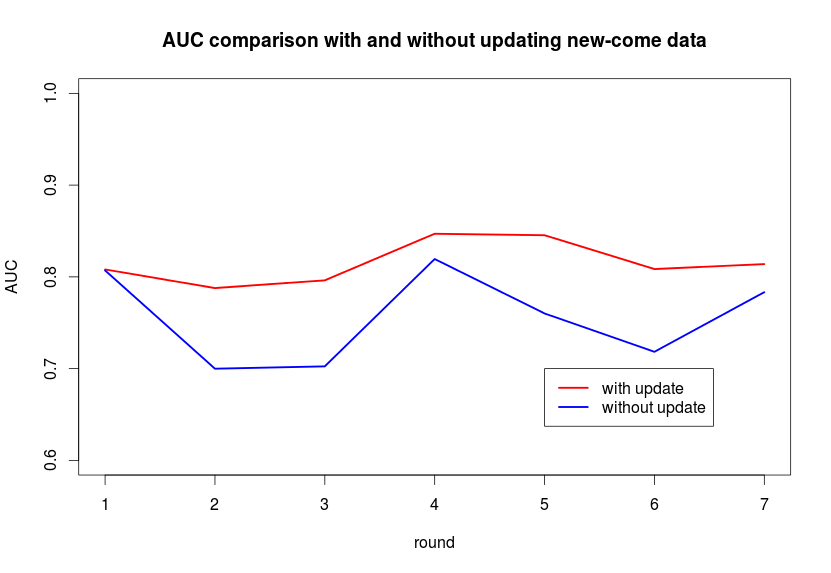
\includegraphics[width=13cm]{countupdate.png}
\end{figure}
 





\end{document}
